% !TeX spellcheck = en_US
% !TEX root = ../thesis-example.tex
%
\chapter{Extending Reality}
\label{sec:extendingreality}

\cleanchapterquote{You are an aperture through which the universe is looking at 
and exploring itself.}{Alan W. Watts}{(Philosopher)}

The well known urban legend of "L'Arriv\'ee d'un train en gare de La Ciotat" in 
which a train arrives at the La Ciotat station, is, that "the audience was so 
overwhelmed by the moving image [...] coming directly at them that people 
screamed and ran to the back of the room". \cite{wiki:train:2017} With that a 
new medium was born, which matured into a new art form of film and movies.
\newline
The most important takeaway is, that with this short clip alone, a door beyond 
still images and their limited depiction of motion has been opened. Video 
imagery changed our imagination and allowed for a new communication form, 
inviting into an animated, moving world. There have been great achievements in 
the last century in motion video production with a great amount of visual 
trickery for composing more realistic and imaginative video content. With the 
help of Computer Generated Imagery (CGI) blurs the boundaries between real 
acting and virtual recreation so far, that it is almost impossible to 
differentiate between real world video capture and 3D recreated imagery in high 
budget productions.

\section{Motion Video Production \& Computer Generated Imagery}

Producing motion video has come a long way and a sufficient history of it would 
be far out of scope for this thesis. Concentrating on key aspects of 
composition techniques might give an appropriate overview to range where Mixed 
Reality takes its inspiration from.

Way before digital imaging processing took over production sets similar 
problems as discussed in this thesis had to be solved, in example how an actor 
can be captured without a back- or foreground and how he would then be 
integrated into an imaginative set. Today, modern action movies don't even 
necessarily capture the actor but his movements, which then will be 
artificially rendered with help of CGI.

\subsection{History of Green \& Blue Screen Productions}

Production set theory is beyond the scope of this thesis, but green- and blue 
screen production has first and foremost a simple reasoning: Green and blue are 
two of the three color triplets that resemble a least amount of color found in 
capturing of humans - and to a certain extent any flora or fauna. Since chroma 
keying (see Ch. \ref{sec:chromakey}) takes color distance as general basis, 
production environments use green screen keying in varying forms. Next to 
$\Delta E$, which will be discussed further, another approach is the 
calculation of fore- and background color spaces and separation of them. The 
latter solution is computationally intense and not suitable for runtime 
applications. \cite{disney:unmixing:2017}
\newline
Green boxes also abuse a correlating advantage that the human eye is most 
susceptible to green (cf. figure \ref{fig:greenscreen:stimula}b), allowing for 
a visual high color range and an ability to differentiate between many shades of
green. Experiments on color range have been done since 1942, trying to 
understand gambit ranges and color differentiation of human vision (figure 
\ref{fig:greenscreen:stimula}a). These experiments concluded that eye cone 
cells see a blending range of wavelengths at different intensities, giving the 
green vector space its highest perceptible range. \cite{MacAdam:1942}

\begin{figure}[htbp]
	\caption{Previous color reception research}
	\label{fig:greenscreen:stimula}	
	\centering
	\begin{subfigure}[t]{.35\textwidth}
		\centering
		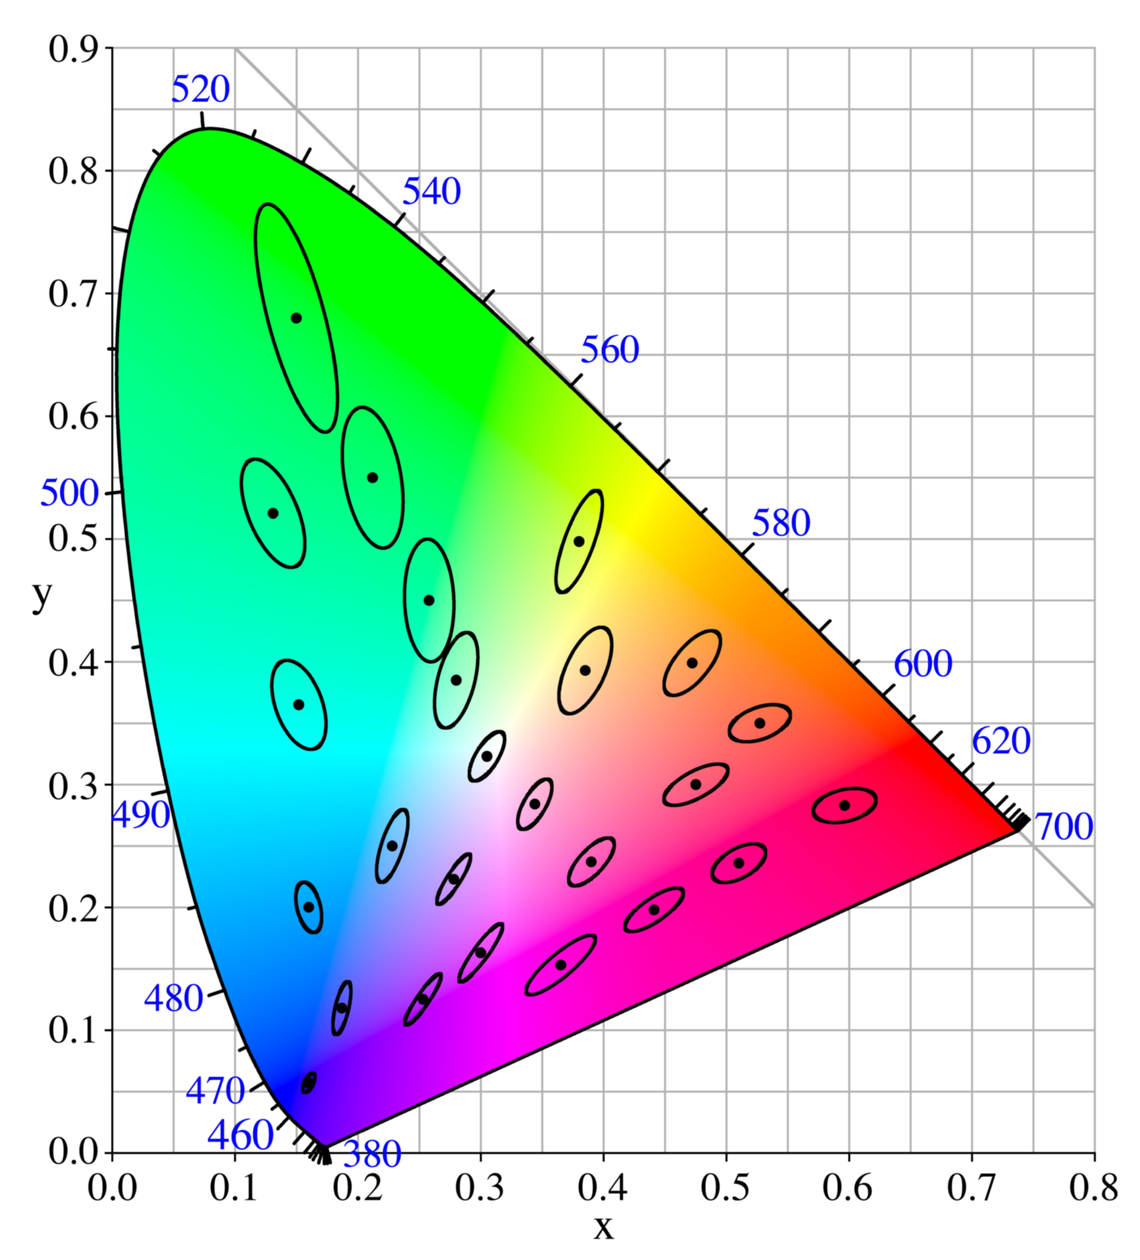
\includegraphics[width=\textwidth]{_external/media/CIExy1931_MacAdam.png}
	\caption{MacAdam ellipses on 1931 standard chromaticity diagram 
		\cite{wiki:macadam:2017}}
	\end{subfigure}
	\begin{subfigure}[t]{.5\textwidth}
		\centering
		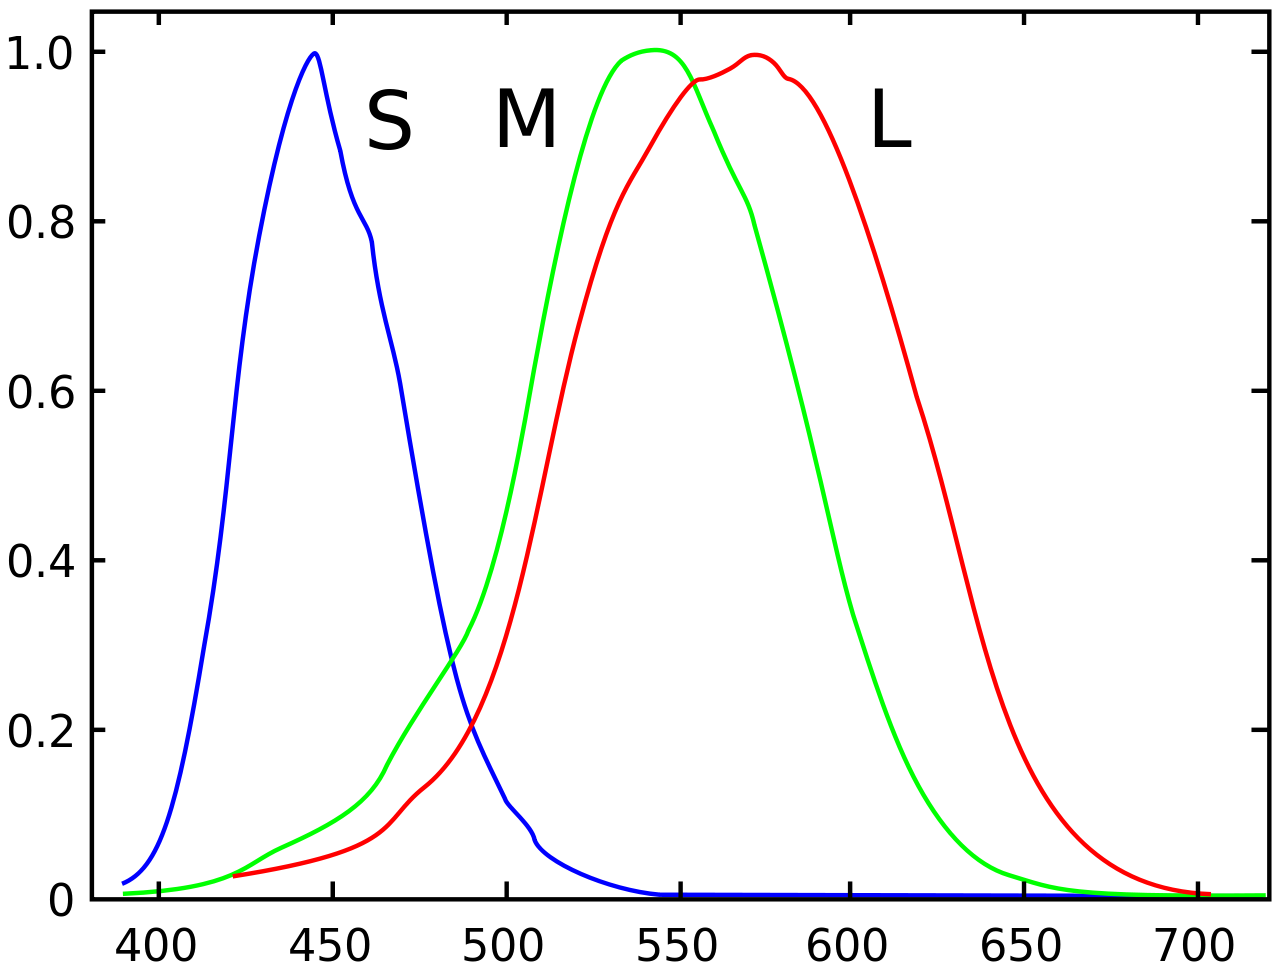
\includegraphics[width=\textwidth]{_external/media/1280px-Cones_SMJ2_E.png}
		\caption{Normalized responsivity spectra of human cone cells, S, M, and 
		L types after Wyszecki et. al \cite{wiki:Wyszecki:2017}. Notice the 
		overlap between M and L cones.}
	\end{subfigure}
\end{figure}
Most consumer cameras - and even most production cameras - use dot-matrix 
sensors with a weighted ration of green (4), red (2) and blue (2) pixels, 
called Bayer pattern \cite{kodak:bayer:1976}, giving it - similar to human 
vision - a high color vector space. Green is generally easier to light, 
illuminate and adjust over blue screens. Small irregularities, for example 
through uneven lightning or crinkles in the material, can be spotted and 
adjusted easily by the production crew.
\newline
The quality of input footage makes a big difference in separating back- and 
foreground, hence a well lit and adjusted set is a good backbone for well 
working chroma keying.

\section{What's VR - Differentiation of AR, VR \& MR}

In search of an appropriate abbreviation for computer-enhanced real-time 
imagery a recent addition is "XR", where \textit{X} is a letter of your choice. 
Definitions are getting more diluted and generally describe a technique, rather 
than an apparent effect by now.

\begin{figure}[htb]
	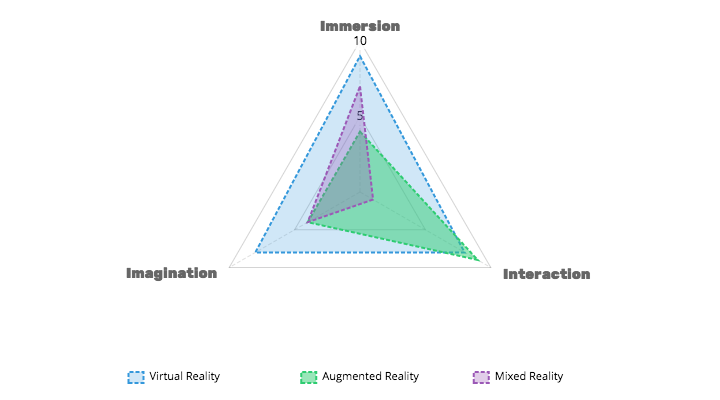
\includegraphics[width=\textwidth]{gfx/ext-reality/i3-triangle.png}
	\caption{I\textsuperscript{3} Triangle - figurative quantization of 
		different reality extending methods}
	\label{fig:xr:i3-triangle}
\end{figure}
Augmented Reality (AR) is a concept to augment real-world imagery with 
additional information and interactive objects. It used to be called Mixed 
Reality\cite{satoh:case:1998} \cite{tamura:mixed-reality:2001}, merging 
real-world imagery with 3D objects but has slowly adapted to AR, since they 
both described the same concept. It ranges from very simple devices displaying 
data in the field of view of a user up to full augmentation, displaying 3D 
models overlaying on real world objects. This can be done ranging from Pepper's 
Ghost projections, augmenting video --- a famous example is the rather 
successful "Pokémon GO" ---, up to the Microsoft HoloLens, that has sensors for 
a wide range of spatial mapping, spatial anchoring and distant field 
calculation.

Virtual Reality is a concept usually done by stereo projection of a 3D 
environment inside a Head-Mounted Display. It takes a user out of the current 
room and sets him into a complete new, virtual reality - hence the origin of 
its name. HMD hardware ranges from the simplistic Google Cardboard --- using a 
smart phone as display device --- to the Samsung GearVR --- similarly uses a 
smart phone as display driver --- up to the Oculus Rift and HTC Vive --- which 
are driven by a mid- to high range PC. The latter two products offer room-scale 
experiences where an user is able to move freely in his play space (basically a 
tacked bounding volume) and allows for six degrees of freedom (\gls{6dof}) 
tracking.

Mixed Reality is an extension of Virtual Reality, allowing bystanders to get an 
impression of the virtual 3D environment around an actor. By reproducing 
virtual projection parameters of a 3D environment, it is possible to place a 
real world camera feed at the right position inside the 3D scene. This 
yields a combined application of Augmented and Virtual Reality techniques. A 
production environment can be achieved with a \gls{6DOF} HMD and additional - 
either user or tracking input for positional and rotational parameters for the 
real-world camera. 

\section{Immersion vs. Communication}

Virtual Reality, as previously mentioned in \ref{sec:intro:outline}, is very 
immersive but the experience is hard to imagine without wearing an HMD 
yourself. Additionally, VR doesn't offer any way to allow observers a similar 
experience as the VR actor.
\newline
A very obvious problem begins with interaction. A VR user doesn't always need 
to see his hands to interact with a scene due to the natural way of holding VR 
controllers in his hands and directly translating controller interaction to the
virtual environment. However an outside viewer does not see the actors hands 
and will not understand any actions performed by the user if he doesn't see the 
virtual hands. Any usage context that happens off-screen cannot be communicated 
and therefore will be lost.

Mixed Reality merges the actors and virtual realities context, allowing outside 
bystanders a comparable window into the actors experienced world. In fact, 
initial promotional material for the HTC Vive showed mixed reality footage, 
produced by one VR computer and a secondary composition PC 
\cite{valve:mr-production:2016}. Its setup is comparable to the one in this 
thesis and differs by composition techniques and by using more than one 
software context, done by outputting a rendered image of the virtual scene and 
compositing it on another system.

\subsection{Evolution of Virtual Reality Footage}

Originally, VR footage consisted of the output that was sent to the headset 
(fig. \ref{fig:evolution:steps}a), including image transformation that needs to 
be done to correct the headset lenses\footnote{this is referred to as "Barrel 
Distortion"} - this distorted dual image is very hard to follow, as it adds two 
ambiguous images and also has a high distortion. Since the direct feed to an 
HMD is used, any translation of the headset's position is visible, which 
results in a jittery and unnatural looking motion feed.

\begin{figure}[htbp]
	\caption{Evolution of VR presentations over the recent years}
	\label{fig:evolution:steps}
	\centering
	\begin{subfigure}[t]{.45\textwidth}
		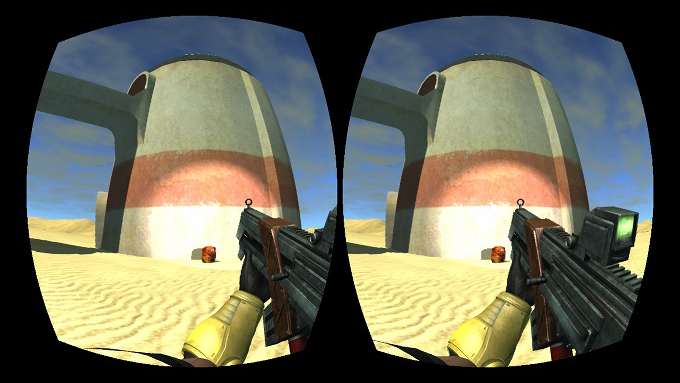
\includegraphics[width=\textwidth]{gfx/evolution/torque3d-bdist.png}
		\caption{Distorted direct dual output to a Oculus 
		DK1\cite{wyand:torqu3d:2013}.}
	\end{subfigure}
	\begin{subfigure}[t]{.45\textwidth}
		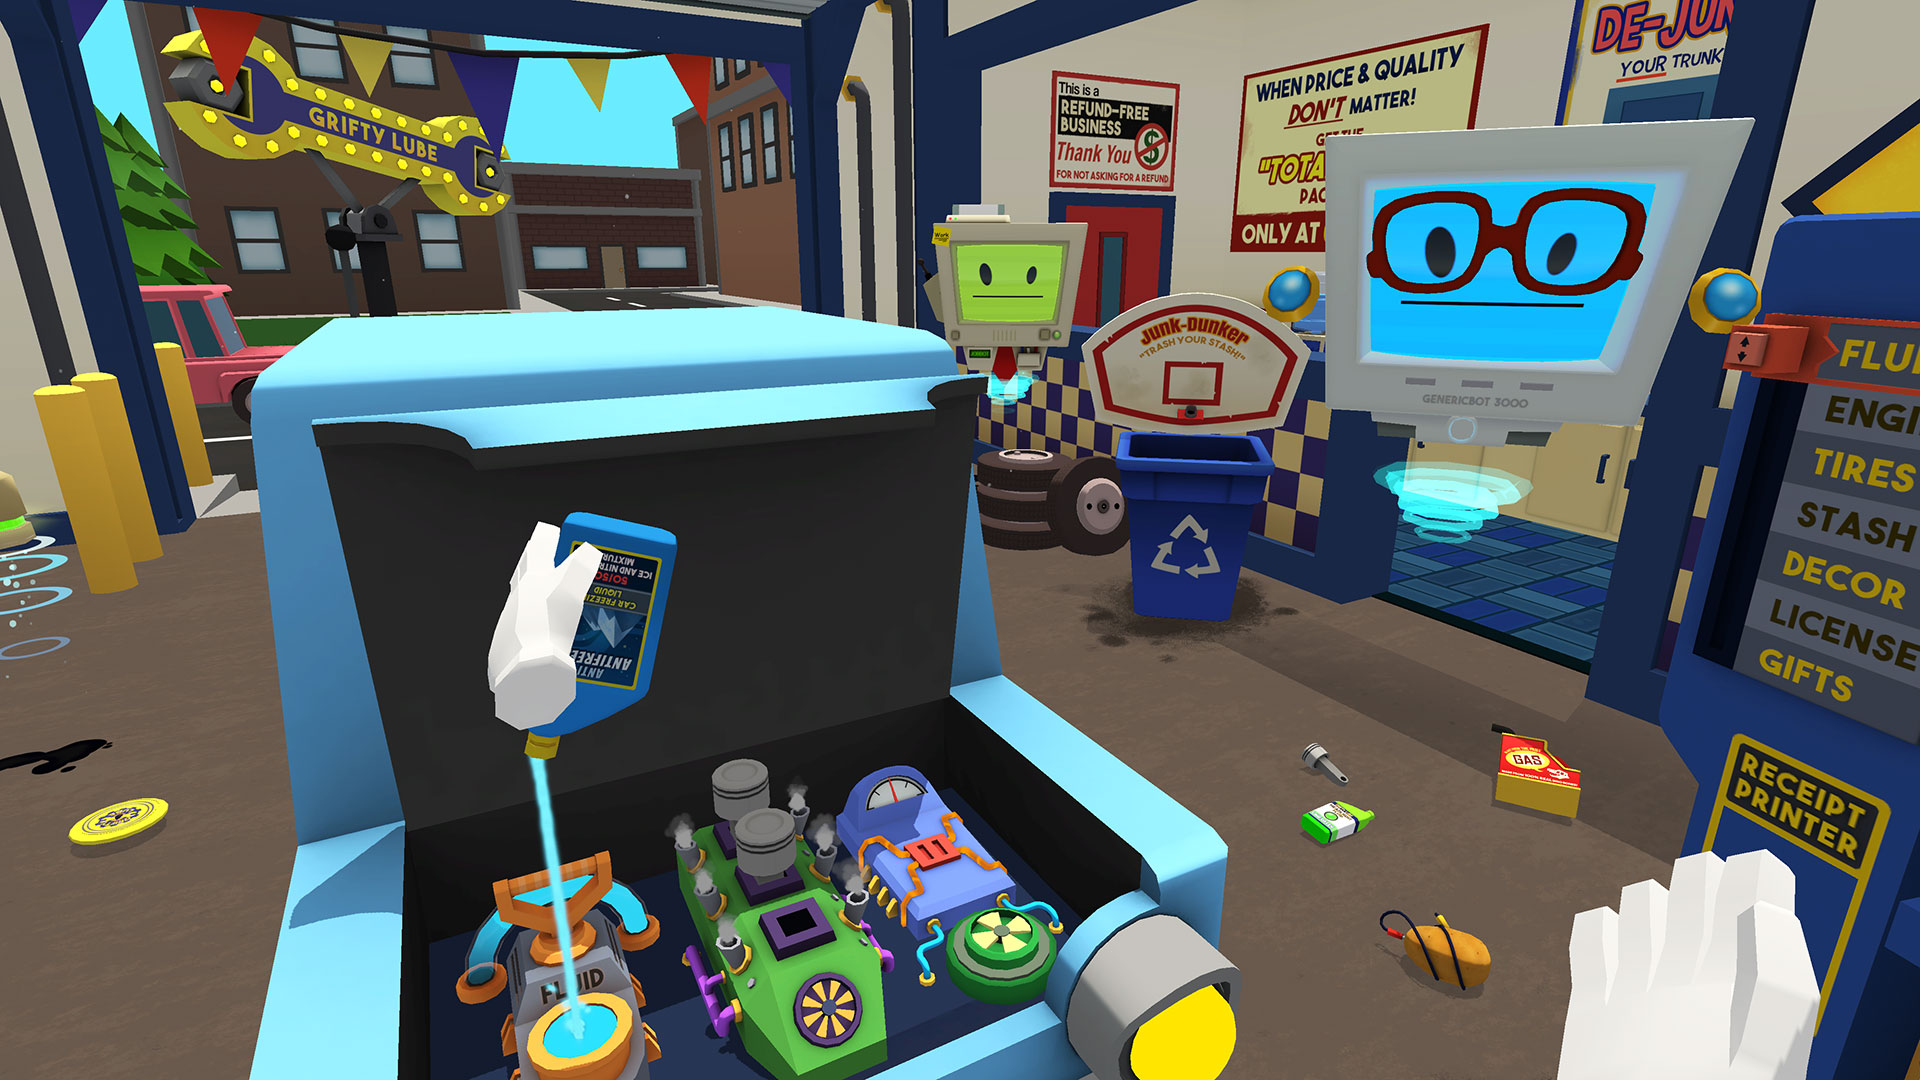
\includegraphics[width=\textwidth]{gfx/evolution/owlch-car.png}
		\caption{A first person, single screen output is an improvement, but is 
			hard to follow in motion.}
	\end{subfigure}
	\begin{subfigure}[t]{.45\textwidth}
		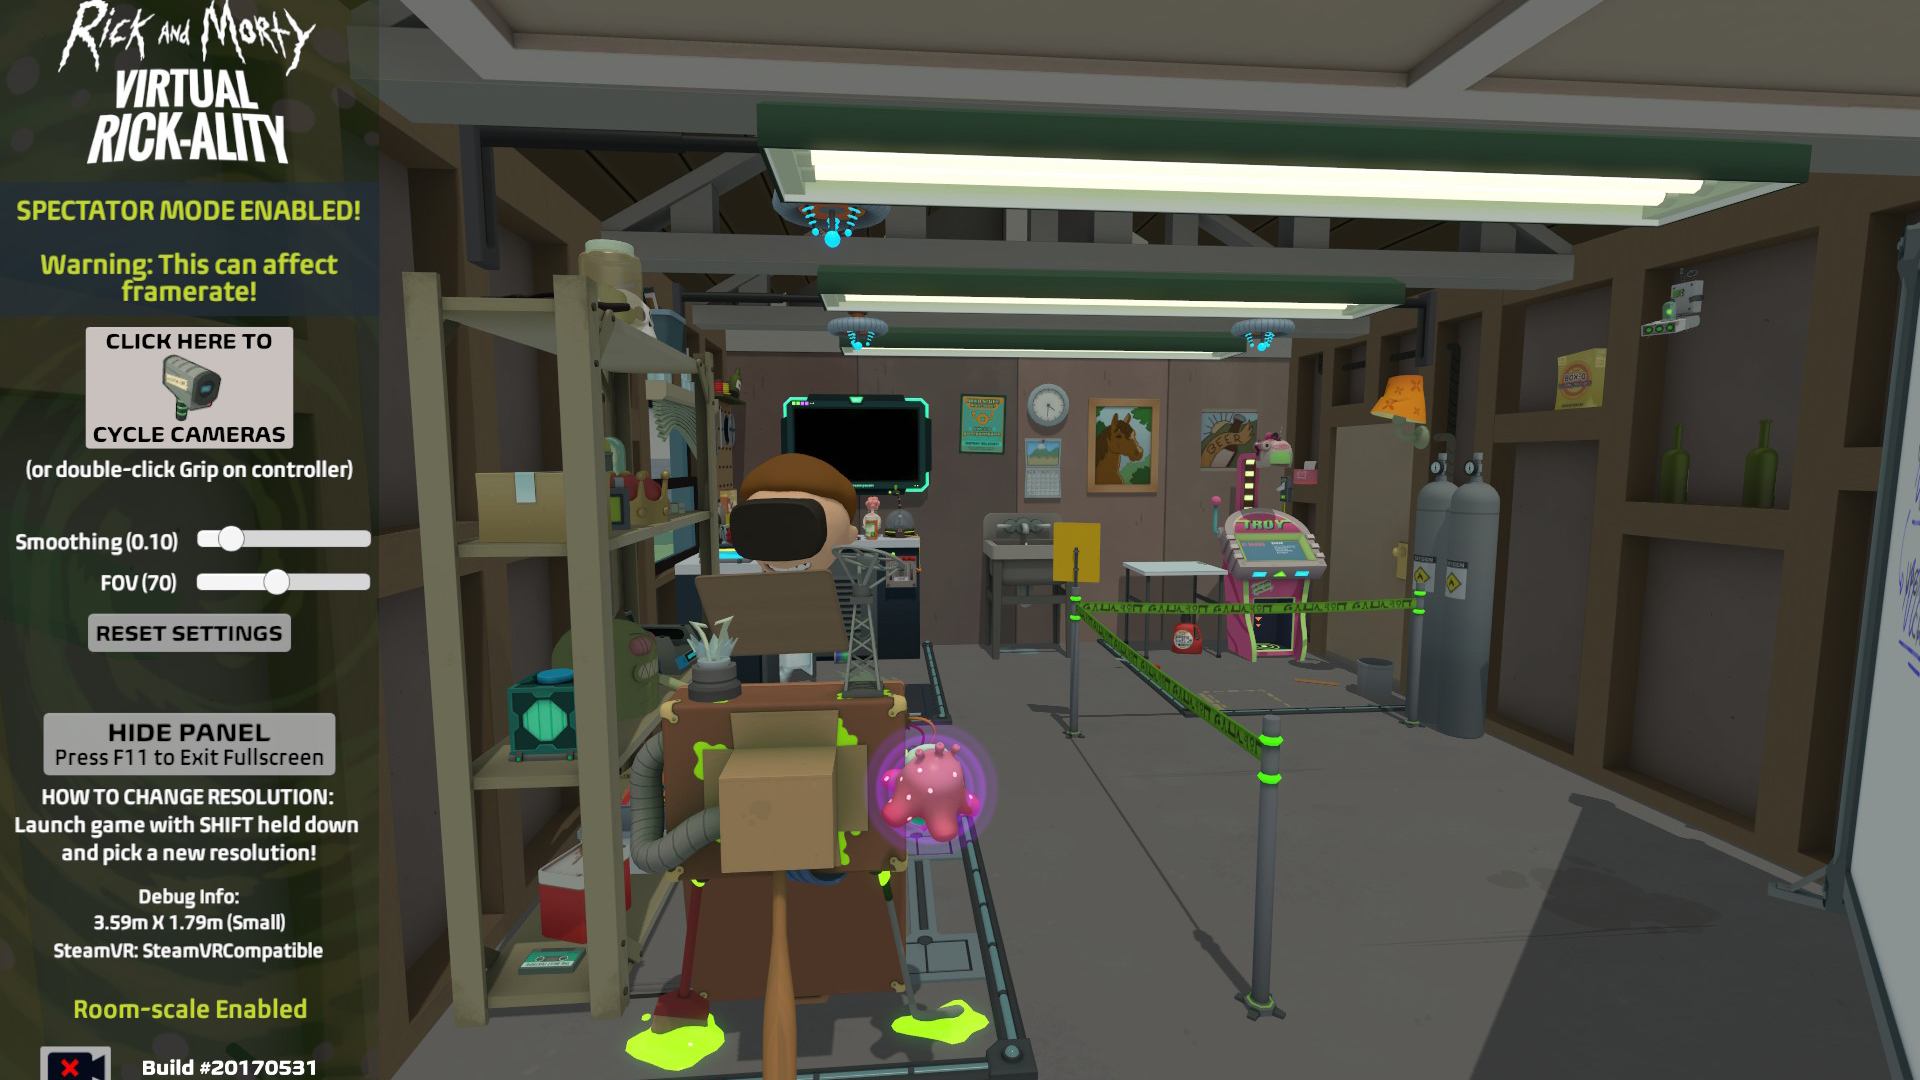
\includegraphics[width=\textwidth]{gfx/evolution/cctv.png}
		\caption{"Rick and Morty: Virtual Rick-Ality" allows outside observers 
			to control mounted CCTV cameras to observe the actors interaction.}
	\end{subfigure}
	\begin{subfigure}[t]{.45\textwidth}
		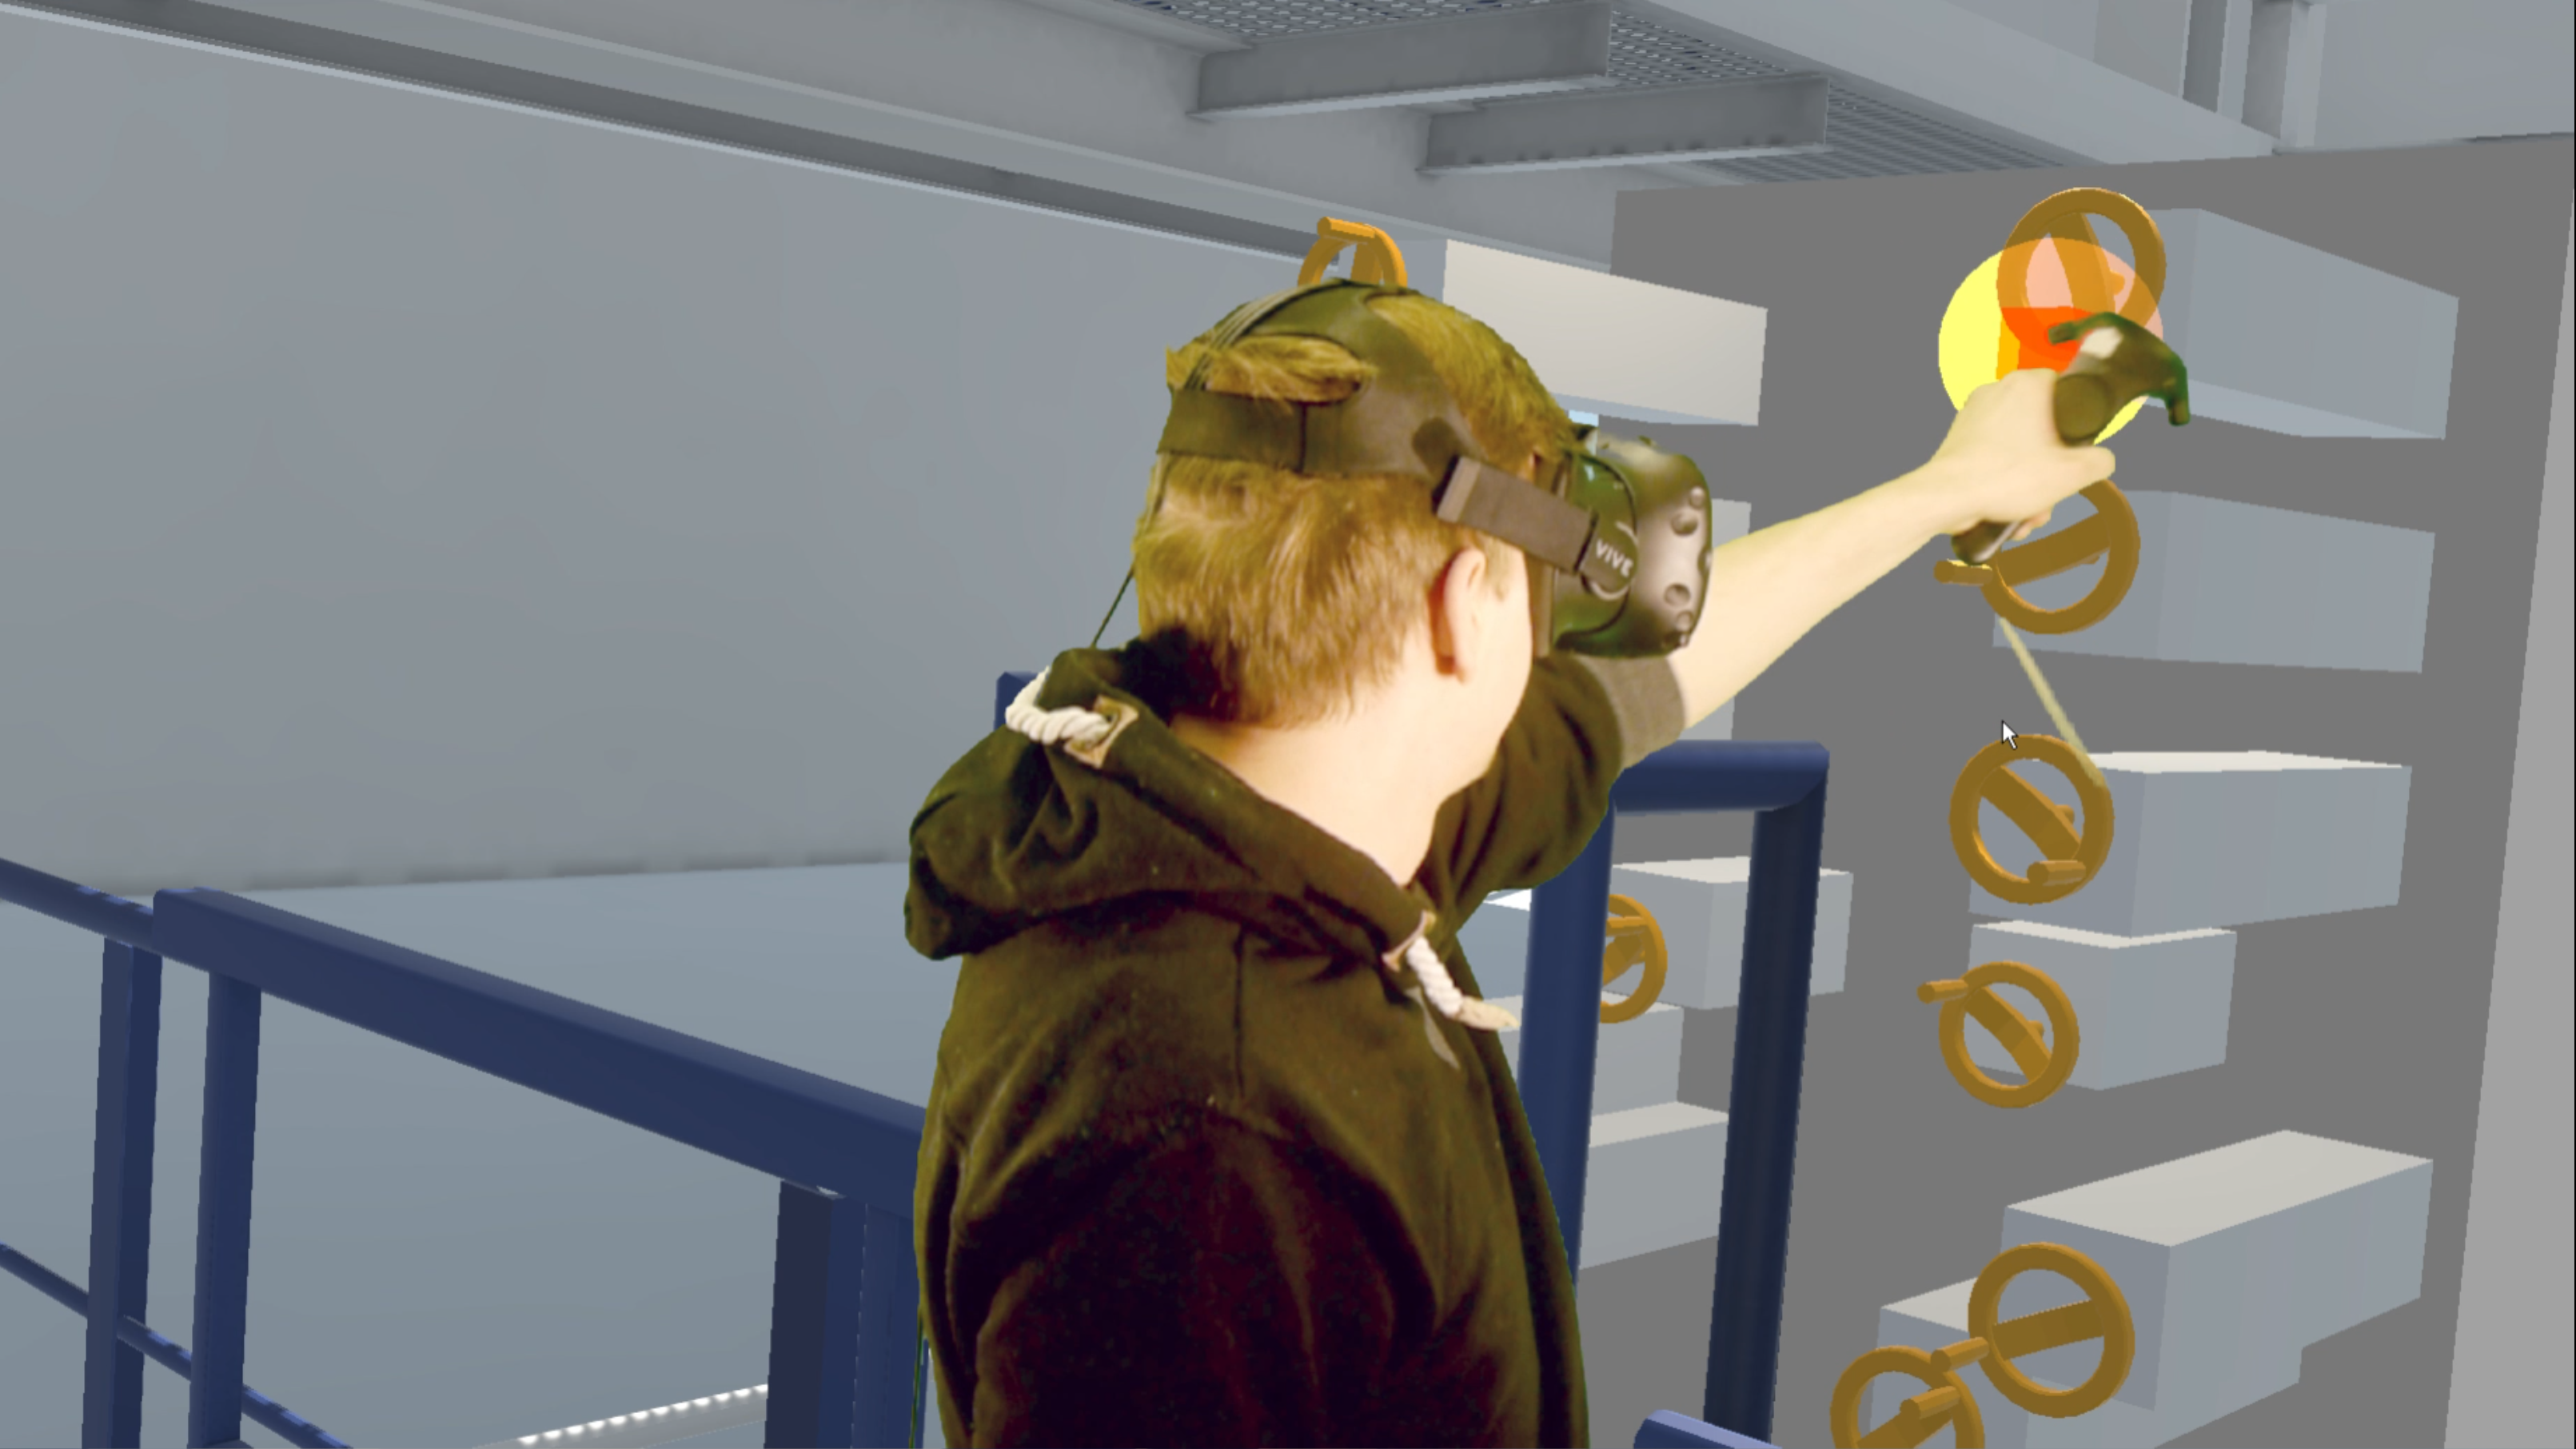
\includegraphics[width=\textwidth]{gfx/evolution/mr-action.png}
		\caption{Recontextualizing the VR actor with the virtual environment 
		makes usage context simpler to understand and easier to follow as 
		observer.}
	\end{subfigure}
\end{figure}

A next step was to render one eye in fullscreen of the attached monitor and do 
all image transformations (mainly crop and distort) after rendering it (fig. 
\ref{fig:evolution:steps}b), allowing bystanders to get a clear first-person 
image of the actor's experience. Additionally, as a secondary camera, a 
dampened movement can be set to mitigate jittery motion. As previously pointed 
out, this works but sometimes loses interaction context, especially when no 
hands are visible. 
\newline
Then there is currently only one game, Rick and Morty: Virtual Rick-ality, that 
has an optional CCTV feature enabled (fig. \ref{fig:evolution:steps}c), in 
which third persons can control a variety of mounted, virtual cameras and 
follow the actors interaction with the 3D environment. This VR actor is then 
replaced with an avatar to visualize what how he is interacting with the 
scenery.
\newline
Finally, there is mixed reality, where the VR actor is placed in context of 
the virtual reality scene (fig. \ref{fig:evolution:steps}d). This has been done 
previously by post-production for trailers and allows for a better 
understanding between virtual interaction and real-actor motion. With its help 
it is possible to invite third-person viewers into the VR experience in a 
natural way.

\section{Mixed Reality and its Use Cases}

First and foremost, Mixed Reality allows re-contextualizing the VR actor with 
the environment. It is far more interesting watching a user interacting with 
the world he is surrounded by than just seeing his first person action. This 
allows i.e. for better Trailer production, that gives a good impression of the 
VR game.
\newline
This back propagation of an actor into a world gives Mixed Reality an 
unexplored field of VR experiences, which can be driven by very classic motion 
video production --- and this idea isn't brand new either. Motion capturing, 
for example in game development, usually translate instantly an actors motion 
into a live 3D rendering, in which the visual performance can be rated by the 
director of this scene.
\newline
"Circle of Saviour" is currently a moving exhibition piece where a VR user can 
slay trolls and goblins, which is viewed as a kind of live news broadcast by 
observers. It is more attention-gathering than regular VR experiences, which 
only allow for a single person view. 
\newline
Going further, without a director on set, this re-contextualizing expands the 
possibilities for multi-user experiences - since the VR actor can be surrounded 
by a complete fictional world, he can play a performance that is directed by a 
crowd.

These cases just highlight a very small amount of new possibilities by 
real-time Mixed Reality productions but highlight how diverse the integration 
of motion video theory back into Virtual Reality can be.

\section{Current State of Mixed Reality Production}

There have been an increasing number of presentations for mixed reality setups. 
To sort this thesis into the current state of production environments, it is 
necessary to look at other approaches and their differences to the proposed 
solution in this thesis.

\subsection{SteamVR \& Oculus SDK Plugins}

Both SteamVR and Oculus SDKs supply plugins to enable mixed reality capturing. 
These systems approach the problem similarly by compositing an incoming video 
stream directly at the current position of a registered camera tracker, thus 
failing to accommodate for different input latencies from the motion video 
feed, yielding an inconsistent visual performance. Oculus states on their 
manuals, that these are currently only intended "for proof-of-concept, 
troubleshooting, and hobby use." \cite{oculus:mr-setup:2017}
\newline
In addition, SteamVRs solution supports video-only composition with a 4K 
HDMI output - which in turn means that the signal has to be captured on an 
external device and has to be composited on a secondary system. The 
configuration parameters are "barebones" at best and yielding good results is a 
matter of the best possible studio setup capture.

\subsection{Fantastic Contraption}

The game "Fantastic Contraption" from 2016 allows livestreamers to do a video 
composition for mixed reality. While this approach allows to mitigate video 
input delays it cannot have a free moving camera with an additional motion 
tracker (see fig. \ref{fig:mrproduction:fcontraption}).

\begin{figure}[htb]
	\centering
	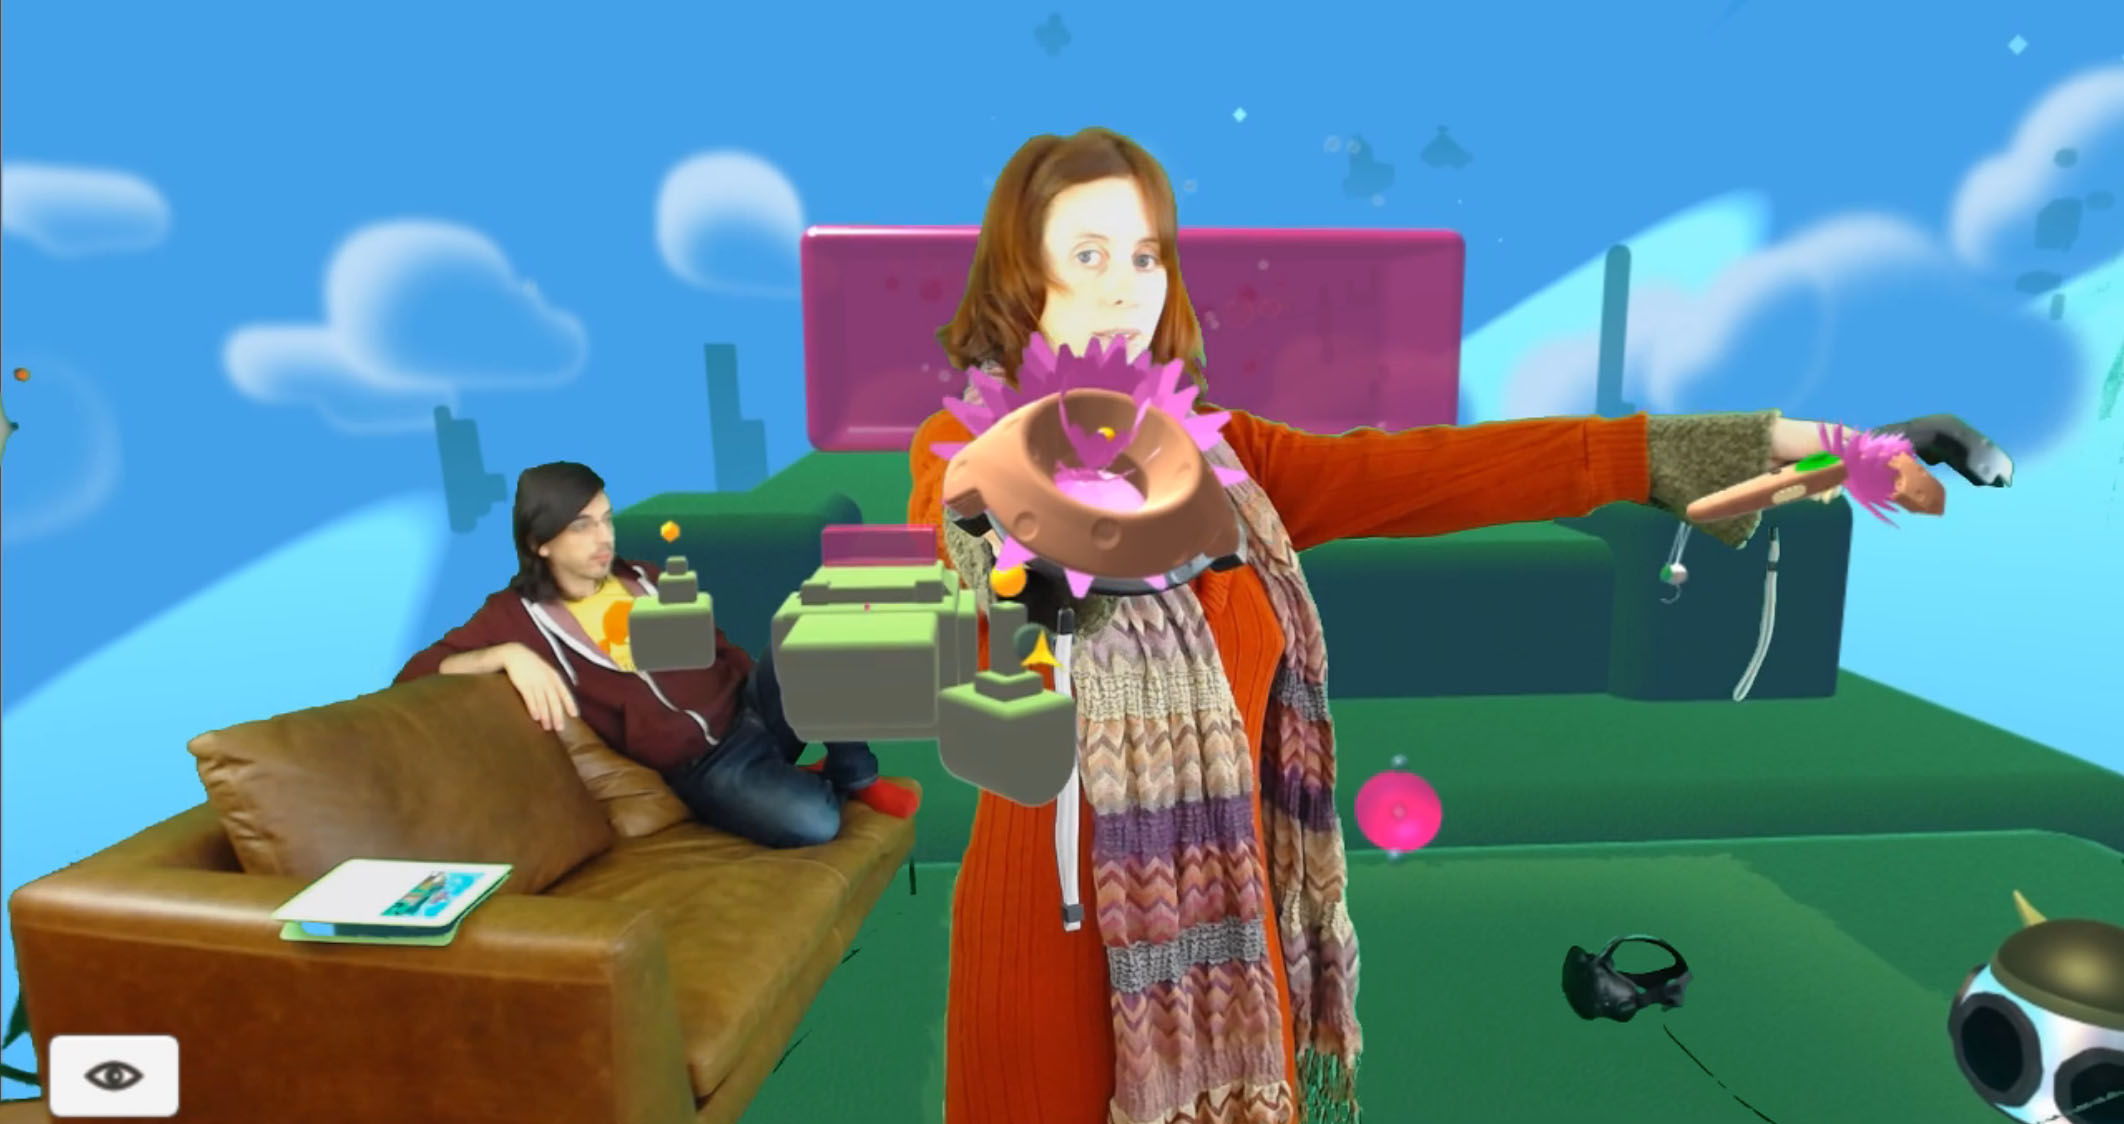
\includegraphics[width=\textwidth]{_external/media/fcontraption-mr.jpg}
	\caption{Mixed Reality in Fantastic 
	Contraption\cite{northway:fcontraption:2016}}
	\label{fig:mrproduction:fcontraption}
\end{figure}

"Fantastic Contraptions" trailers also show another approach by replacing the 
actor with an avatar by basically rendering a certain depth and then placing 
real-world camera footage as background. With such a system any live video 
background removal is not necessary and real world footage of the actor is 
lost. The game's trailer composition has been achieved in post production. 
\cite{gartner:cinematography:2017}

\subsection{Owlchemy Labs Mixed Reality}

Owlchemy Labs is a VR game studio located in Austin, Texas. They're working 
on VR experiments and use similar techniques discussed in this paper. Their key 
difference in visual reproduction is by using a stereoscopic camera to record 
an actor and can reproduce the actors depth per pixel, allowing for more 
complex fore- and background separation for a more accurate visual 
reproduction as seen in figure \ref{fig:mrproduction:owlchemy}.

\begin{figure}[htb]
	\centering
	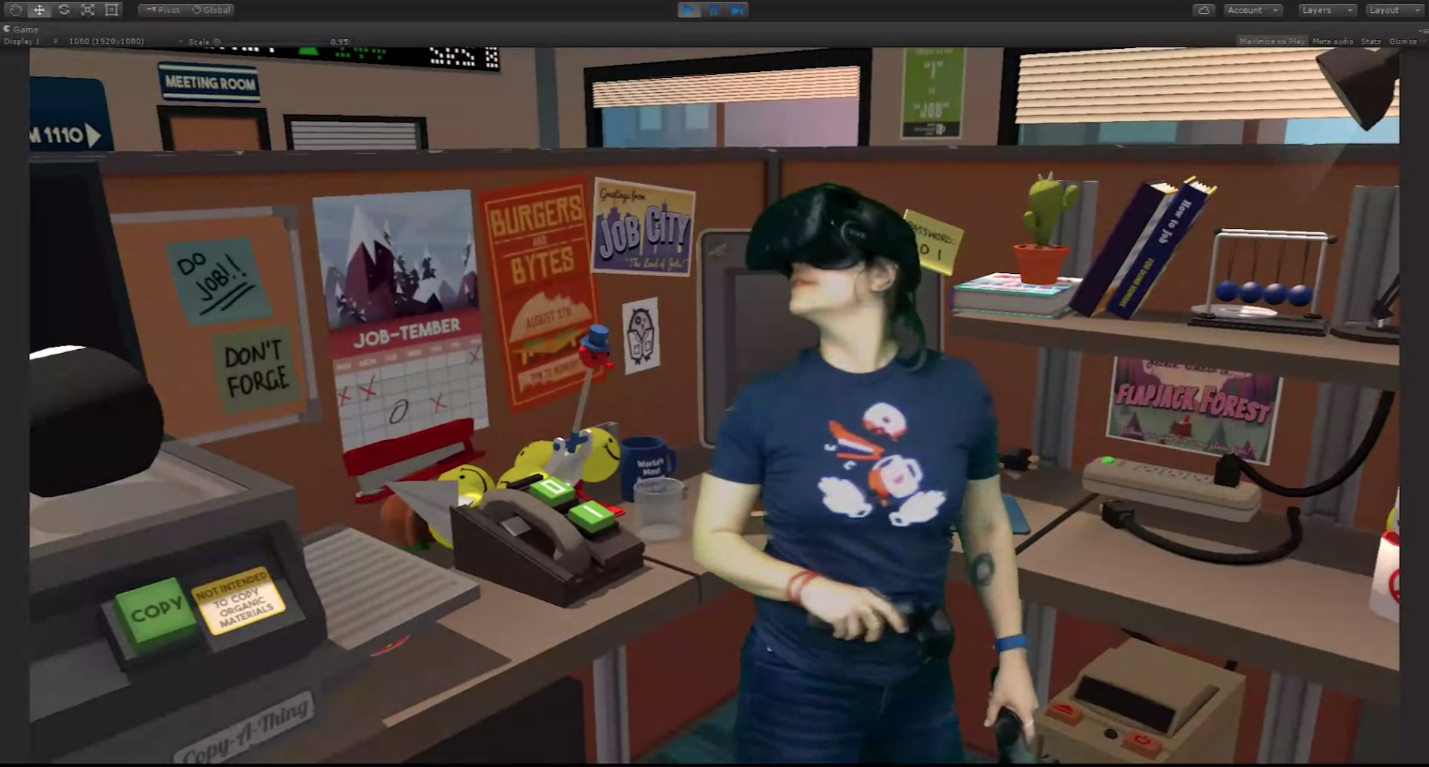
\includegraphics[width=\textwidth]{_external/media/owlch-mr.png}
	\caption{Owlchemy's Mixed Reality Setup\cite{owlchemy:mr:3:2017}}
	\label{fig:mrproduction:owlchemy}
\end{figure}

While Owlchemy Labs announced real-time mixed reality compositing, there hasn't 
been a shipped product or update for one of their games that allows for live 
mixed reality capture\cite{owlchemy:mr:3:2017}.

\newpage
\subsection{Apple WWDC17}

Apple presented a real-time mixed reality showcase done on their computer 
systems on their annual keynote "WWDC17" (see fig. 
\ref{fig:mrproduction:apple}). It is driven by Unreal Engine and 
uses also similar techniques as discussed in this thesis. That presentation is 
currently the best live performance of mixed reality with a high quality chroma 
keying, depth reconstruction and high fidelity graphics. There is no technical 
information available yet\cite{ilmxlab:mr-demo:2017}.

\begin{figure}[htb]
	\centering
	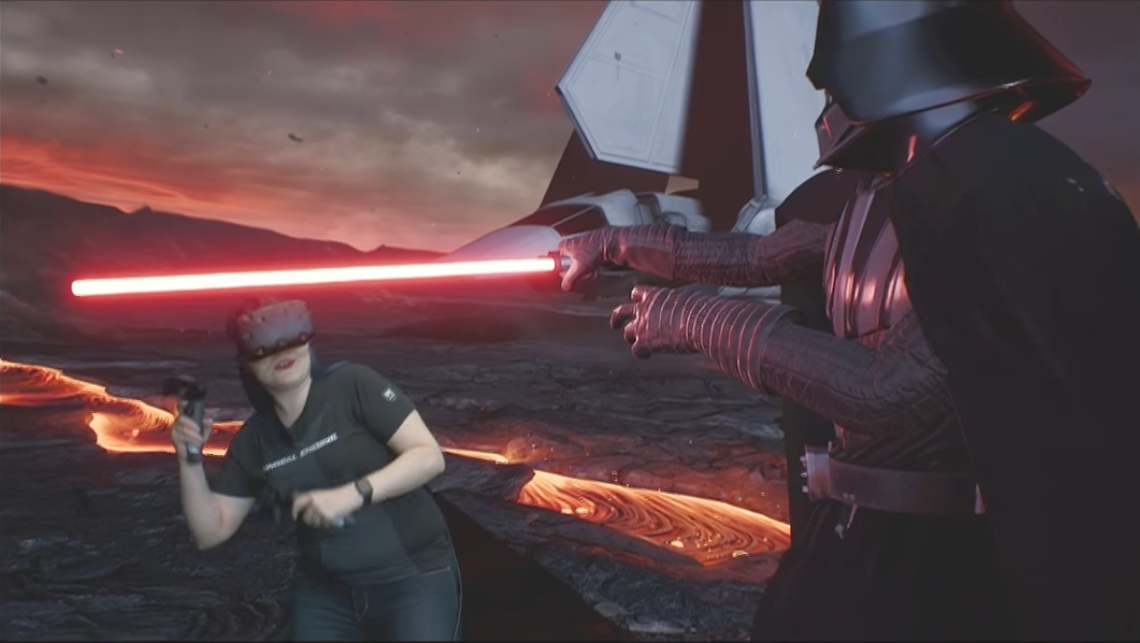
\includegraphics[width=\textwidth]{_external/media/apple-mr.png}
	\caption{Screenshot from the Apple WWDC17 
	demonstration\cite{ilmxlab:mr-demo:2017}}
	\label{fig:mrproduction:apple}
\end{figure}